% TikZ source for figures/fig_pipeline.pdf
%
% Aidan directive 2026-04-19 (fifth pass):
%   - Tighter spacing across the whole diagram.
%   - Arrow from the protocol spec goes into EVERY verifier via its
%     own enabling step. The mid-step box names the concrete
%     transformation we had to do so that verifier could be applied
%     (Lean encoding, Dafny transcription, SV refinement, Hypothesis
%     strategies, CPU simulator build).
%   - The 5 verifier outputs feed "cross-check agreement", which
%     returns feedback to the spec (dashed, refutation loop).
%   - No text on arrows; the semantics is carried by the box labels.

\documentclass[border=5pt]{standalone}
\usepackage{tikz}
\usetikzlibrary{positioning, arrows.meta, shapes.geometric, fit, calc}

\begin{document}
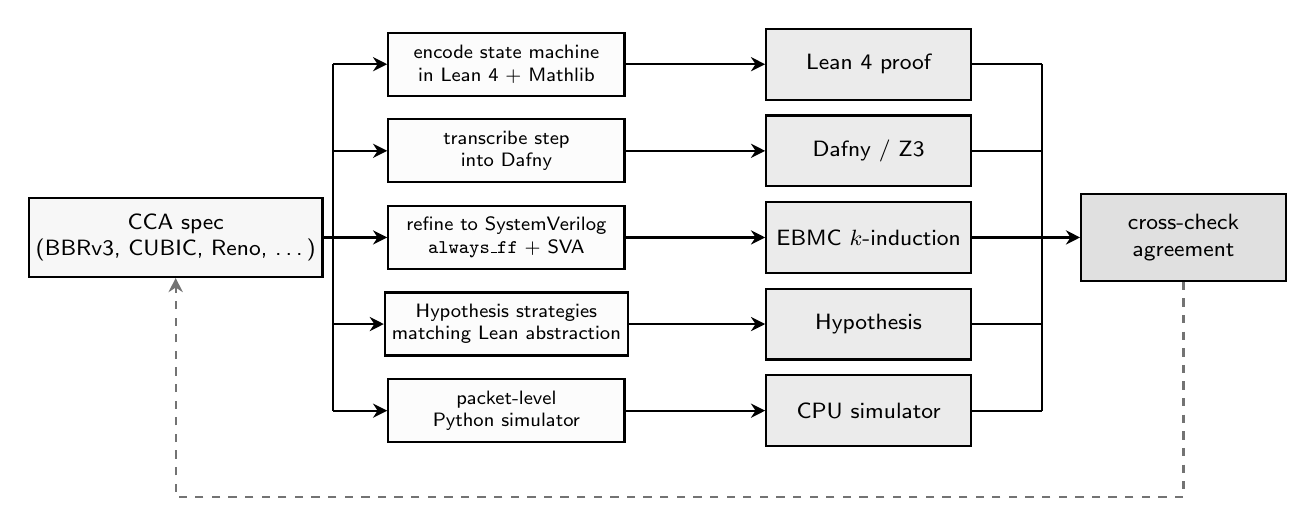
\begin{tikzpicture}[
  font=\sffamily\footnotesize,
  every node/.style={inner sep=2.5pt},
  io/.style={
    draw=black, thick, rectangle, minimum width=22mm, minimum height=10mm,
    align=center, fill=black!3,
  },
  midstep/.style={
    draw=black, thick, rectangle, minimum width=30mm, minimum height=8mm,
    align=center, fill=black!1, font=\sffamily\scriptsize,
  },
  verifier/.style={
    draw=black, thick, rectangle, minimum width=26mm, minimum height=9mm,
    align=center, fill=black!8,
  },
  verdict/.style={
    draw=black, thick, rectangle, minimum width=26mm, minimum height=11mm,
    align=center, fill=black!12,
  },
  arr/.style={-{Stealth[length=1.8mm,width=1.8mm]}, thick},
  feedbackarr/.style={-{Stealth[length=1.8mm,width=1.8mm]},
                      thick, dashed, draw=black!55},
]

% ── Row y-positions (5 rows, 11mm apart) ───────────────────────────
\def\rA{22mm}
\def\rB{11mm}
\def\rC{0mm}
\def\rD{-11mm}
\def\rE{-22mm}

% ── Column x-positions ─────────────────────────────────────────────
\def\cSpec{0mm}
\def\cMid{42mm}
\def\cVer{88mm}
\def\cVerdict{128mm}

% ── Input spec ─────────────────────────────────────────────────────
\node[io] (spec) at (\cSpec,\rC) {CCA spec\\(BBRv3, CUBIC, Reno, \ldots)};

% ── Five mid-step "enabling" boxes (column 2) ──────────────────────
\node[midstep] (mLean)  at (\cMid,\rA) {encode state machine\\in Lean 4 + Mathlib};
\node[midstep] (mDafny) at (\cMid,\rB) {transcribe step\\into Dafny};
\node[midstep] (mEBMC)  at (\cMid,\rC) {refine to SystemVerilog\\\texttt{always\_ff} + SVA};
\node[midstep] (mHyp)   at (\cMid,\rD) {Hypothesis strategies\\matching Lean abstraction};
\node[midstep] (mSim)   at (\cMid,\rE) {packet-level\\Python simulator};

% ── Five verifiers (column 3) ──────────────────────────────────────
\node[verifier] (vLean)  at (\cVer,\rA) {Lean 4 proof};
\node[verifier] (vDafny) at (\cVer,\rB) {Dafny / Z3};
\node[verifier] (vEBMC)  at (\cVer,\rC) {EBMC $k$-induction};
\node[verifier] (vHyp)   at (\cVer,\rD) {Hypothesis};
\node[verifier] (vSim)   at (\cVer,\rE) {CPU simulator};

% ── Cross-check (column 4) ─────────────────────────────────────────
\node[verdict] (agree) at (\cVerdict,\rC) {cross-check\\agreement};

% ── Spec -> each mid-step (fan-out) ────────────────────────────────
% Use a short vertical bus at x = 20mm to make it clear the five
% paths all originate from the same spec, without overlapping arrows.
\coordinate (busT) at (20mm,\rA);
\coordinate (busB) at (20mm,\rE);
\draw[thick] (spec.east) -- (20mm,\rC);
\draw[thick] (busT) -- (busB);
\draw[arr] (20mm,\rA) -- (mLean.west);
\draw[arr] (20mm,\rB) -- (mDafny.west);
\draw[arr] (20mm,\rC) -- (mEBMC.west);
\draw[arr] (20mm,\rD) -- (mHyp.west);
\draw[arr] (20mm,\rE) -- (mSim.west);

% ── Mid-step -> verifier (straight right) ──────────────────────────
\draw[arr] (mLean.east)  -- (vLean.west);
\draw[arr] (mDafny.east) -- (vDafny.west);
\draw[arr] (mEBMC.east)  -- (vEBMC.west);
\draw[arr] (mHyp.east)   -- (vHyp.west);
\draw[arr] (mSim.east)   -- (vSim.west);

% ── Verifier -> cross-check (fan-in) ───────────────────────────────
\coordinate (cbusT) at (110mm,\rA);
\coordinate (cbusB) at (110mm,\rE);
\draw[thick] (cbusT) -- (cbusB);
\draw[thick] (vLean.east)  -- (110mm,\rA);
\draw[thick] (vDafny.east) -- (110mm,\rB);
\draw[thick] (vEBMC.east)  -- (110mm,\rC);
\draw[thick] (vHyp.east)   -- (110mm,\rD);
\draw[thick] (vSim.east)   -- (110mm,\rE);
\draw[arr] (110mm,\rC) -- (agree.west);

% ── Refutation feedback: agreement -> spec (below the rows) ────────
% Dashed arrow routed under the verifier row so nothing overlaps.
\draw[feedbackarr] (agree.south) |- (\cSpec,-33mm) -| (spec.south);

\end{tikzpicture}
\end{document}
